\chapter{Existing Systems} \label{chapter:systems}
Mapping is not a very new task: digital mapping gained momentum with the growing popularity for personal navigation devices (like TomTom in 2007, \cite{guardian:tomtom}). However this has all been focused on roads with no consideration to features around the roads. There are however three major organisations who have considered feature and location classification using differing methods:











\section{Google Maps}
Supposedly the market leader in mapping, Google Maps is the most used mapping tool in the world with 1 in 7 people from the entire planet using it at least once a month! Google maps collects it data from a large pool of sources:
\begin{itemize}
 \item \textbf{Map Partners} - Organisations that provide the ``most comprehensive and authoritative data sources" \citep{google:makeusof}
\item \textbf{Satellites} - Until 2014, Google did not own satellites. By investing in satellite businesses, they are provided with images in return \citep{google:satellites}
\item \textbf{Location Services} - By having access to every user's location, users can passively crowd source data.
\item \textbf{Street View} - Ingeniously Google have found many ways of extracting information about features from the images taken on the ground via roaming vehicles.
\end{itemize}.

These are combined in many ways to produce the maps provided on maps.google.com. Google keeps most of these implementations private. However, their engineers often provide hints on the methods used. A technique similar to our own system is the use of satellite imagery for cartography. The image on the left of figure \ref{fig:googlemaps} shows a first layer of processing of a satellite image. 

\begin{figure}[H]
    \centering
    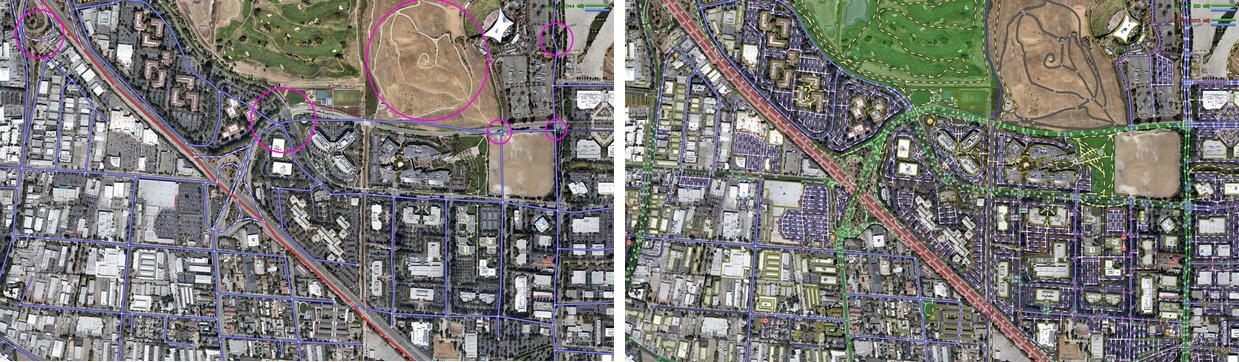
\includegraphics[width=\textwidth]{figs/2/googlemaps}
    \caption{Google Maps Satellite Conversion}
    \label{fig:googlemaps}
\end{figure}

Through the usage of the locations services and manual human editing \citep{google:wired}, the image on the right of figure \ref{fig:googlemaps} is generated. These are then classified by the army of google users. The majority of the work that has been completed was through sheer man-power. Modern techniques are not disclosed to the public. 

A common issue with Google's imagery is that the longitude and latitudes are often incorrect, since the scale in the image is unreliable. The accuracy of labels also reduces the further a tag is from a populated area. Google formally makes no claims on the accuracy of their systems, claiming that their measurements “are provided for entertainment only” \citep{google:forum}.

This leaves Google Maps as a novel system with little industrial usage potential. With methods kept formally hidden and implementation only suggested at through blogs and interviews, Google Maps is not a direct competitor nor useful to design decisions. 







\newpage
\section{Terrapattern} \label{section:existing:terrapattern}
\href{http://www.terrapattern.com/}{Terrapattern} is considered the main competitor in this field. Currently in alpha, it has many of the same features as required by the client. Using the google maps API it has classified every minor tile within the bounds of six cities in the USA and Berlin. It is an open source project available on \href{https://github.com/CreativeInquiry/terrapattern}{github}. 

\begin{figure}[H]
    \centering
    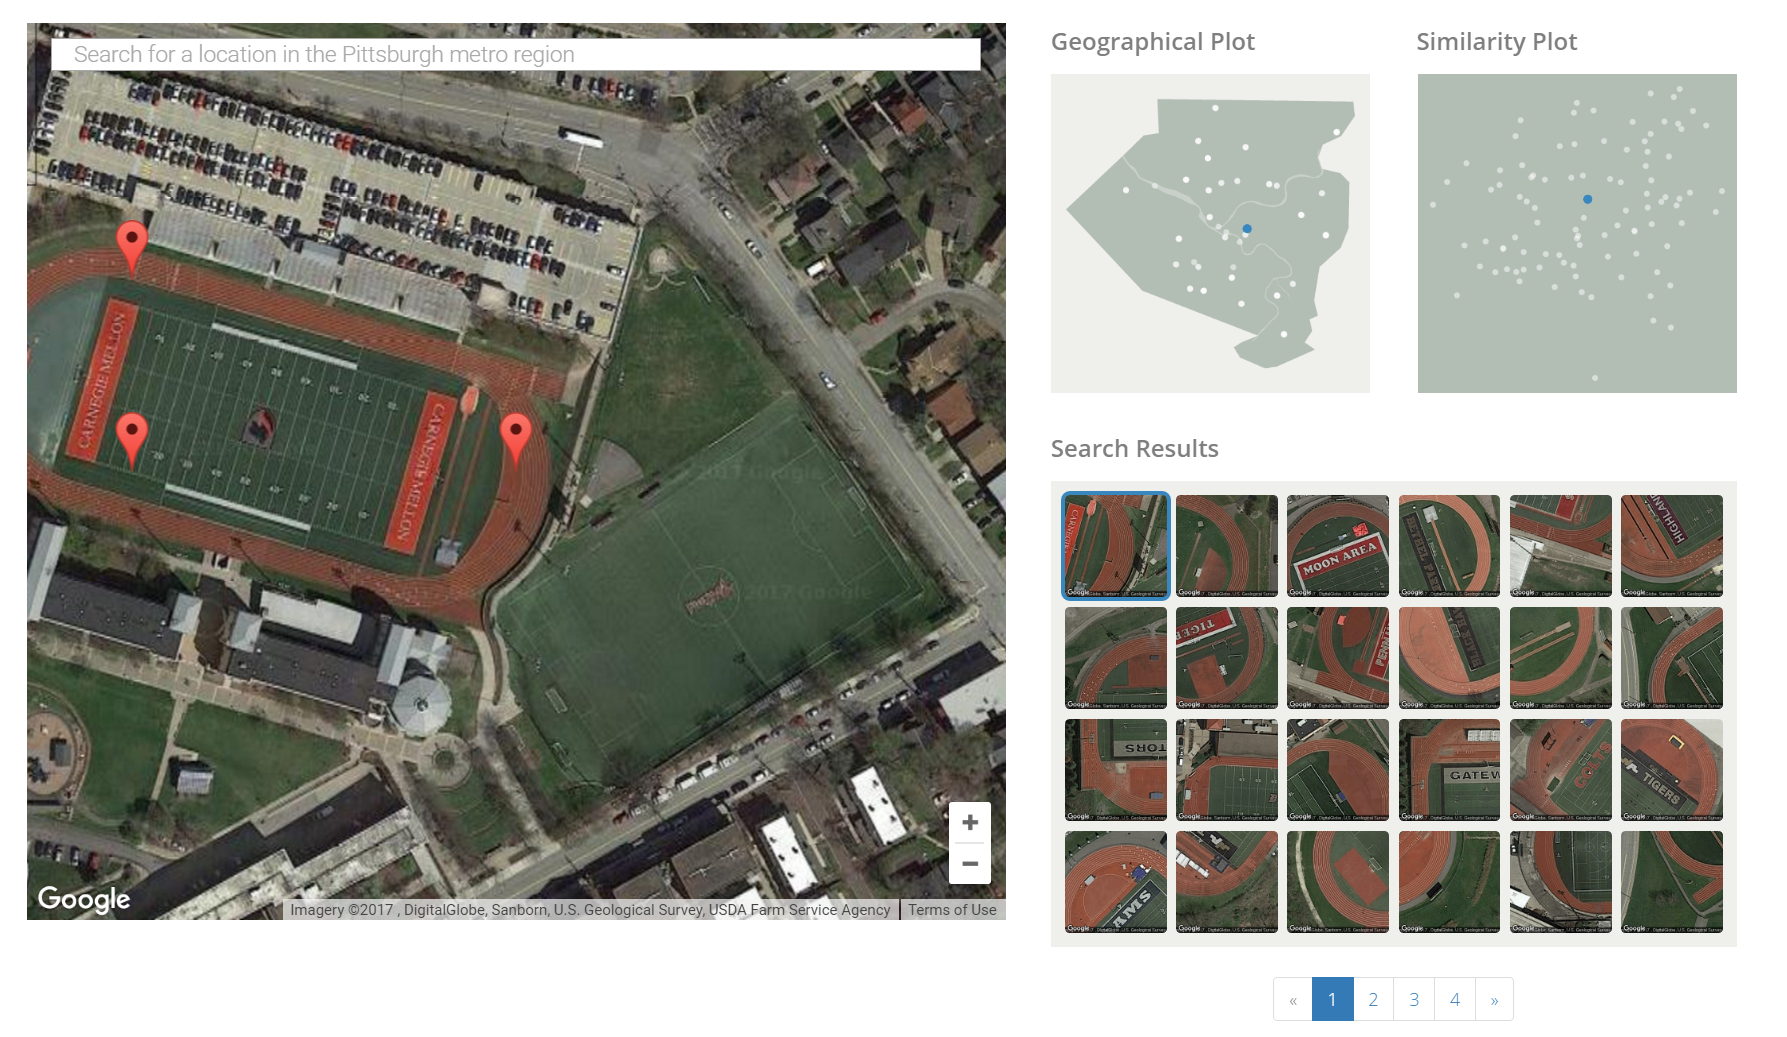
\includegraphics[width=\textwidth]{figs/2/terrapattern}
    \caption{Terrapattern finding corner running tracks in Pittsburgh (USA)}
    \label{fig:terrapattern}
\end{figure}

\subsection*{How it works}
For each city within Terrapattern, an extremely large polygon is selected off of google maps and is tiled. Many labelled features are taken from the OpenStreetMap dataset and processed through a deep neural network (DNN), training it. Then every tile of the city is processed through that DNN in order to classify it \citep{terrapattern:howitworks}.

\subsection*{Pros}
Terrapattern has a very large collection of feature types, with an intriguing precision (e.g. purple tennis courts rather than just tennis courts). Its clear minimaps allow for density of features to be easily observed. Users can search for specific features. This technique is fantastic for identifying and finding similar odd objects, like their example of finding cargo boats or corners of running tracks (figure \ref{fig:terrapattern})

\subsection*{Cons}
The developers of Terrapattern have admitted this is a only a prototype, explaining the reason why it is wrought with flaws. Due to the tiling, it cannot handle the fuzzy border issue that is often accompanied with uniform tiling (The fuzzy border issue is expanded on in section \ref{section:fuzzy}), causing rather unintelligent classifications, as can be seen in figure \ref{fig:bad_terrapattern}. Due to the subtle angle in the streets of San Francisco, identical housing is not identically labelled and roads with trees cannot be continuously discovered. This issue is propagated throughout the map. 


\begin{figure}[H]
    \centering
    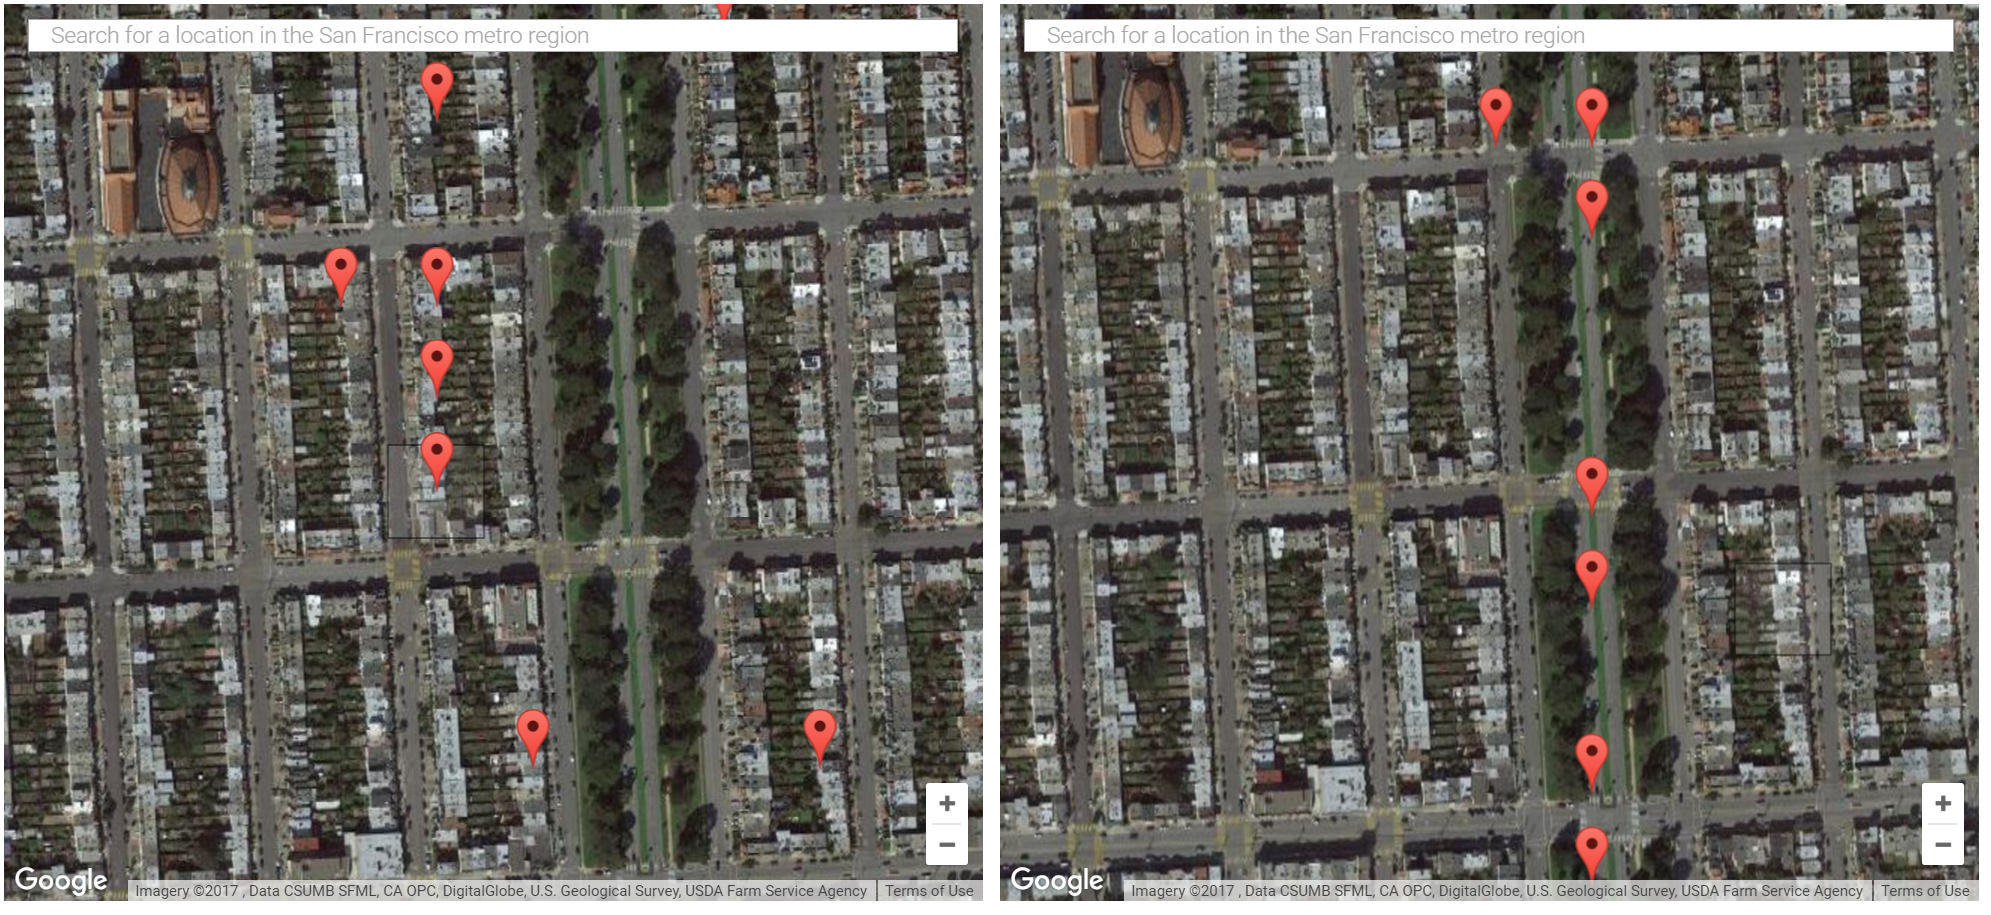
\includegraphics[width=\textwidth]{figs/2/bad_terrapattern}
    \caption{Fuzzy Border Issue in Terrapattern}
    \label{fig:bad_terrapattern}
\end{figure}

The results of Terrapattern are static. They do not allow for any corrections or additions to the map. This prevents the previously mentioned errors from being fixed. This is a serious issue with the semi-unsupervised nature of the model, resulting in the errors remaining there.

The technical components of Terrapattern are evidently strong, however according to their system it is considerably slow. The process of training the DNN took 5 days, and resulted in a top-5 error rate of 25.4\% (\cite{terrapattern:howitworks}), which is unfortunately not that accurate. 

\subsection*{Evaluation}
Terrapattern's approach to the problem is very good. The technical approach and tools themselves are novel. However, the lack of supervised learning and support for supervised learning holds it back. In the context of Ordnance Survey, this makes the method of learning used by Terrapattern near useless as the world is not a series edge cases, but actually full of conformity that this tool cannot easily handle.



